% =====================================================================
% Figure: Tightness degradation vs perturbation budget epsilon.
% Visual companion to tab:tightness_eps (experiments.tex). Data are the
% mean tightness ratios (actual / first-order-predicted shift) across
% 10 seeds for each dataset at eps in {0.01, 0.05, 0.10, 0.20}.
%
% Design notes (revision pass):
%   - Two background bands encode the qualitative regimes:
%       * vertical light-grey band: "operational regime" (eps in [0.10,0.20])
%       * horizontal light-green band: "tight regime" (y in [0.99,1.03])
%     Bands carry their own labels, so the prior "perfect first-order"
%     text no longer has to live UNDER the data lines.
%   - "perfect first-order (y=1)" is now a callout tag anchored to the
%     right end of the y=1 reference line, with a white-fill bbox so it
%     sits CLEAN on top of the green band.
%   - Citation graphs use SOLID lines (cool palette); product graphs use
%     DASHED lines (warm palette) -- visual grouping mirrors the two
%     qualitatively different tightness behaviours.
%   - Right-end numeric value tags at eps=0.20 give the reader the exact
%     terminal tightness without having to eye-trace to the y-axis.
% =====================================================================

\documentclass[tikz,border=4pt,11pt]{standalone}
\usepackage[T1]{fontenc}
\usepackage{mathptmx}
\usepackage{tikz}
\usepackage{pgfplots}
\pgfplotsset{compat=1.18}
\usetikzlibrary{calc}
\usepackage{xcolor}
\usepackage{amsmath, amssymb}
\renewcommand{\familydefault}{\rmdefault}

% Okabe-Ito (colourblind-safe). Shared with all other figures.
\definecolor{okBlue}{HTML}{0072B2}
\definecolor{okOrange}{HTML}{E69F00}
\definecolor{okGreen}{HTML}{009E73}
\definecolor{okVermilion}{HTML}{D55E00}
\definecolor{okPink}{HTML}{CC79A7}
\definecolor{okSkyBlue}{HTML}{56B4E9}
\definecolor{okGrey}{HTML}{888888}

\begin{document}
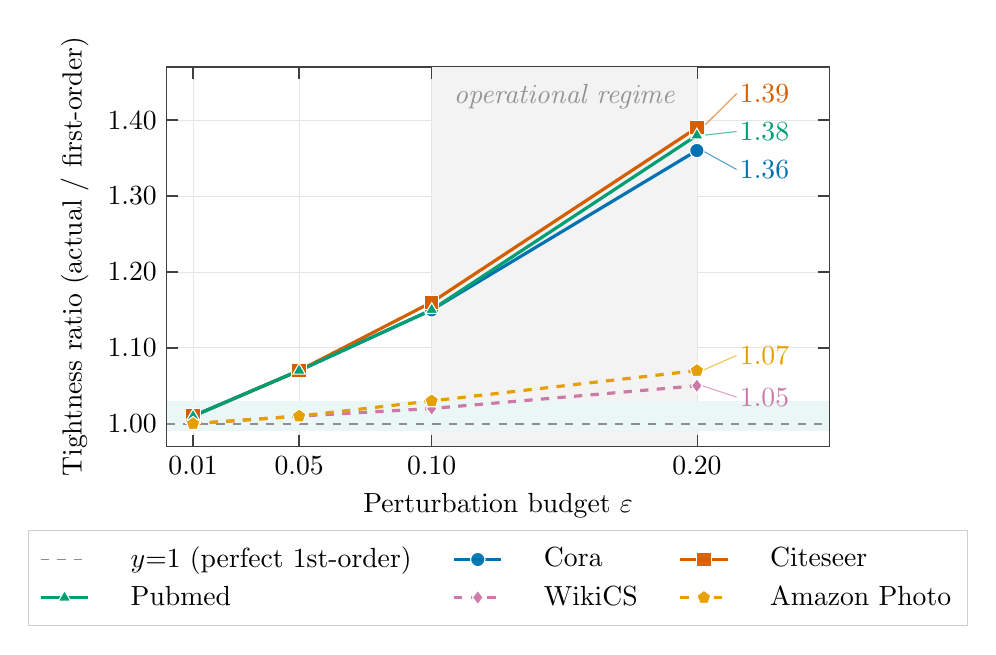
\begin{tikzpicture}[font=\rmfamily]
\begin{axis}[
    width=10.0cm, height=6.4cm,
    xlabel={Perturbation budget $\varepsilon$},
    ylabel={Tightness ratio (actual / first-order)},
    xmin=0, xmax=0.250,
    ymin=0.97, ymax=1.47,
    xtick={0.01,0.05,0.10,0.20},
    xticklabels={$0.01$, $0.05$, $0.10$, $0.20$},
    ytick={1.00,1.10,1.20,1.30,1.40},
    yticklabel style={/pgf/number format/.cd, fixed, precision=2, zerofill},
    grid=major,
    grid style={line width=.25pt, draw=okGrey!22},
    axis line style={line width=0.6pt, draw=black!75},
    tick style={line width=0.6pt, draw=black!75},
    tick label style={font=\normalsize},
    label style={font=\normalsize},
    % Legend lives BELOW the axis as a 3-column horizontal row. Frees the
    % entire plot area for data + annotations and avoids any in-plot
    % overlap with the "operational regime" header at the top of the
    % grey band.
    legend style={
        at={(0.5, -0.22)}, anchor=north,
        font=\normalsize,
        draw=okGrey!40,
        line width=0.4pt,
        fill=white,
        fill opacity=0.95,
        text opacity=1,
        row sep=1pt,
        column sep=0.45cm,
        inner sep=4pt,
        legend columns=3,
    },
    legend cell align={left},
    clip=false,
    every axis plot/.append style={line width=1.15pt, mark size=2.6pt},
]

% --- Background regime bands (drawn FIRST so they sit behind curves) ----
% Vertical grey band: "operational regime" -- where epsilon is actually
% applied in the rest of the paper.
\fill[okGrey!10] (axis cs:0.10, 0.97) rectangle (axis cs:0.20, 1.47);
% Horizontal green band: "tight regime" -- ratio within 3% of unity.
\fill[okGreen!8]  (axis cs:0, 0.99) rectangle (axis cs:0.250, 1.03);

% --- y=1 reference line (perfect first-order prediction) -----------------
% NOT forget plot -- gets a legend entry so the meaning ("perfect first
% order") is conveyed cleanly in the legend instead of an inline label
% that would crowd the chart.
\addplot[okGrey!95, dashed, line width=0.7pt]
    coordinates {(0, 1.0) (0.250, 1.0)};
\addlegendentry{$y{=}1$ (perfect 1st-order)}

% --- Citation graphs (solid lines, cool palette) -------------------------
\addplot[color=okBlue, mark=*,
         mark options={fill=okBlue, draw=white, line width=0.4pt}]
    coordinates {(0.01,1.01) (0.05,1.07) (0.10,1.15) (0.20,1.36)};
\addlegendentry{Cora}

\addplot[color=okVermilion, mark=square*,
         mark options={fill=okVermilion, draw=white, line width=0.4pt}]
    coordinates {(0.01,1.01) (0.05,1.07) (0.10,1.16) (0.20,1.39)};
\addlegendentry{Citeseer}

\addplot[color=okGreen, mark=triangle*,
         mark options={fill=okGreen, draw=white, line width=0.4pt}]
    coordinates {(0.01,1.01) (0.05,1.07) (0.10,1.15) (0.20,1.38)};
\addlegendentry{Pubmed}

% --- Product graphs (dashed lines, warm palette) -------------------------
% 'solid' on mark options keeps the markers themselves crisp despite the
% dashed line.
\addplot[color=okPink, dashed, mark=diamond*,
         mark options={fill=okPink, draw=white, line width=0.4pt, solid}]
    coordinates {(0.01,1.00) (0.05,1.01) (0.10,1.02) (0.20,1.05)};
\addlegendentry{WikiCS}

\addplot[color=okOrange, dashed, mark=pentagon*,
         mark options={fill=okOrange, draw=white, line width=0.4pt, solid}]
    coordinates {(0.01,1.00) (0.05,1.01) (0.10,1.03) (0.20,1.07)};
\addlegendentry{Amazon Photo}

% --- Right-end value annotations at eps=0.20 -----------------------------
% Citation cluster: y values 1.36, 1.38, 1.39 are close together. Fan the
% labels out vertically (1.335, 1.385, 1.435 -- ~0.05 gap each) and add
% short, colour-matched leader lines back to the actual data point so the
% reader can still link each label to its source line.
\draw[okBlue!65, line width=0.4pt]
    (axis cs:0.202, 1.36) -- (axis cs:0.215, 1.335);
\node[font=\normalsize, anchor=west, color=okBlue, inner sep=1pt]
    at (axis cs:0.215, 1.335) {$1.36$};

\draw[okGreen!65, line width=0.4pt]
    (axis cs:0.202, 1.38) -- (axis cs:0.215, 1.385);
\node[font=\normalsize, anchor=west, color=okGreen, inner sep=1pt]
    at (axis cs:0.215, 1.385) {$1.38$};

\draw[okVermilion!65, line width=0.4pt]
    (axis cs:0.202, 1.39) -- (axis cs:0.215, 1.435);
\node[font=\normalsize, anchor=west, color=okVermilion, inner sep=1pt]
    at (axis cs:0.215, 1.435) {$1.39$};

% Product cluster: 1.05 and 1.07 fanned to 1.035 / 1.085 (~0.05 gap).
\draw[okPink!65, line width=0.4pt]
    (axis cs:0.202, 1.05) -- (axis cs:0.215, 1.035);
\node[font=\normalsize, anchor=west, color=okPink, inner sep=1pt]
    at (axis cs:0.215, 1.035) {$1.05$};

\draw[okOrange!65, line width=0.4pt]
    (axis cs:0.202, 1.07) -- (axis cs:0.215, 1.090);
\node[font=\normalsize, anchor=west, color=okOrange, inner sep=1pt]
    at (axis cs:0.215, 1.090) {$1.07$};

% --- Regime-band labels --------------------------------------------------
% "operational regime" sits at the top of the grey band, horizontal.
% (The y=1 dashed reference is labelled in the legend; the green
% tight-regime band's meaning is explained in the caption.)
\node[font=\normalsize\itshape, color=okGrey!90, anchor=north]
   at (axis cs:0.15, 1.46) {operational regime};

\end{axis}
\end{tikzpicture}
\end{document}
